As we create and train the network Dropout layer is used for regularization. 
Using dropout consist in dropping randomly some neuron from the network. 
Those neuron are consider ar "turned off" meaning they won't impact the futur weight updates. \\
While training on one example neuron can co-adapt on becoming really specific to an example. 
Using dropout regularization we prevent then the neuron to co-adapt too much and the network to be less specific and better in generalization. 
Dropout prevent then from overfitting and to be stuck in a local minimum of the error gradient.

\begin{itemize}
\item \textbf{Forward pass :} 

During the forward pass we are modifying the network itself, neuron are dropped from the network with the probability p (and kept with propbability q=1-p) - each neuron has the same probability to be dropped or not. 
To do so we used a a binomial distribution $\mathcal{B}$(N,p) to decide wether a neuron is dropped or not.\\
If we are using dropout during the training phase we need to perform a rescaling (x $\frac{1}{1-p}$) on the neuron in order to make the network operational for testing. 


\item \textbf{Backward pass :} 

During the backpropagation we just need to consider the Dropout, neuron that have been dropped doesn't contribute to further updates, they consquently need to be dropped in the derivative matrix - coresponding weight won't be updated. Therefor mask need to be stored between forward an backward pass to know which neuron have been dropped.

\end{itemize}


\begin{figure}[!ht]
    \centering
    {{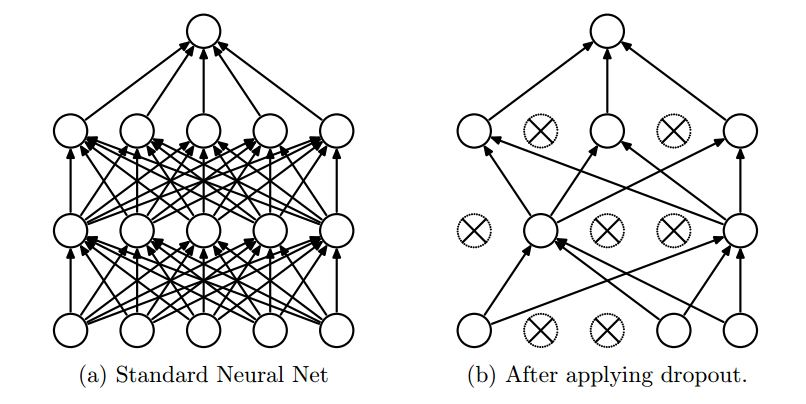
\includegraphics[scale = 0.50]{src/diagrams/dropout.png}}}  
\end{figure}

